% How-to guide: interfacing with the ctrlX Drive Oscilloscope (Scope Capture) service.
% Build: pdflatex scope_capture_how_to.tex  (run twice for the table of contents)
\documentclass[11pt,a4paper]{article}

\usepackage[utf8]{inputenc}
\usepackage[T1]{fontenc}
\usepackage{lmodern}
\usepackage[margin=2.2cm]{geometry}
\usepackage{xcolor}
\usepackage{booktabs}
\usepackage{tabularx}
\usepackage{array}
\usepackage{amsmath}
\usepackage{enumitem}
\usepackage{parskip}
\usepackage{listings}
\usepackage{tikz}
\usetikzlibrary{automata,positioning,arrows.meta}
\usepackage[colorlinks=true,linkcolor=blue!50!black,urlcolor=blue!50!black]{hyperref}

% Let lines break before long monospace names instead of running into the margin.
\setlength{\emergencystretch}{3em}

\definecolor{codebg}{gray}{0.96}
\definecolor{codekw}{rgb}{0.10,0.25,0.60}
\definecolor{codecomment}{rgb}{0.35,0.45,0.35}
\definecolor{codestring}{rgb}{0.60,0.20,0.10}

\lstset{
  basicstyle=\ttfamily\small,
  backgroundcolor=\color{codebg},
  keywordstyle=\color{codekw}\bfseries,
  commentstyle=\color{codecomment}\itshape,
  stringstyle=\color{codestring},
  frame=single,
  rulecolor=\color{gray!40},
  breaklines=true,
  columns=fullflexible,
  keepspaces=true,
  showstringspaces=false,
  xleftmargin=0.5em,
  xrightmargin=0.5em,
}
\lstdefinelanguage{json}{
  morestring=[b]",
  literate={:}{{{\color{codekw}:}}}1 {,}{{{\color{codekw},}}}1,
}

% Short-hands
\newcommand{\dl}[1]{\texttt{#1}}
\newcommand{\capsroot}{\dl{ctrlx-drive-oscope/captures}}
\newcommand{\res}[1]{\texttt{#1}}

\newenvironment{usecase}[1]
  {\subsection{#1}}
  {}
\newcommand{\ucfield}[2]{\par\noindent\textbf{#1:} #2\par}

\title{ctrlX Drive Oscilloscope Service\\[0.3em]\large How-To Guide and Use Cases}
\author{DriveOscopeApp}
\date{\today}

\begin{document}
\maketitle
\tableofcontents
\newpage

%=====================================================================
\section{Overview}
%=====================================================================

The Drive Oscilloscope service runs on a ctrlX CORE as a snap. It records
oscilloscope traces from a ctrlX DRIVE through the Easy Automation Library and
exposes the whole workflow on the ctrlX Data Layer. A client never talks to the
drive directly: it creates a \emph{capture}, fires the trigger, and reads back
the recorded samples, all through Data Layer nodes.

\begin{itemize}[nosep]
  \item One capture configures the oscilloscope of one drive.
  \item Each capture is identified by a server-generated \dl{capture\_id} (UUID).
  \item A capture can record many traces: trigger, read, re-arm, trigger again.
  \item A capture exists until the client deletes it. Captures do not survive a
        service restart.
  \item Only one capture per drive IP address can exist at a time.
\end{itemize}

The data exchanged is defined by two FlatBuffers schemas in
\dl{designDocs/interface/}, which are the source of truth for field names and
types:

\begin{center}
\begin{tabular}{@{}lll@{}}
\toprule
Schema & Root type & Used for \\
\midrule
\dl{scope\_config.fbs}  & \dl{scope\_config.ScopeConfig}  & Body of the create request \\
\dl{scope\_capture.fbs} & \dl{DriveCapture.ScopeCapture} & Recorded trace returned by the service \\
\bottomrule
\end{tabular}
\end{center}

The service registers both as Data Layer types, so tools that understand
Data Layer types (for example the ctrlX CORE Data Layer view) can show the
capture as structured data:

\begin{center}
\begin{tabular}{@{}ll@{}}
\toprule
Type address & Schema \\
\midrule
\dl{types/ctrlx-drive-oscope/scope-config}  & \dl{ScopeConfig} \\
\dl{types/ctrlx-drive-oscope/scope-capture} & \dl{ScopeCapture} \\
\bottomrule
\end{tabular}
\end{center}

%=====================================================================
\section{Prerequisites}
%=====================================================================

\begin{itemize}
  \item The service snap is installed and running on the ctrlX CORE. It needs
        no configuration: it always publishes under \capsroot.
  \item The drive is reachable from the ctrlX CORE over Ethernet at a fixed
        IPv4 address.
  \item The client has Data Layer access to the ctrlX CORE (an app running on
        the CORE, or a remote client with user credentials).
  \item For .NET clients: the \dl{ctrlX-DataLayer} NuGet package from the
        ctrlX Automation SDK, and C\# classes generated from the two schemas
        with \dl{flatc} (see \dl{src/DriveOscope/build-fbs.sh}).
\end{itemize}

\paragraph{Connecting from .NET.}
\dl{new Remote().ToString()} picks the connection automatically: inside a snap
on the ctrlX CORE it returns \dl{ipc://}; anywhere else it builds a TCP
connection string using the given IP address and credentials (factory defaults
\dl{192.168.1.1}, \dl{boschrexroth}/\dl{boschrexroth}, SSL port 443).

\begin{lstlisting}[language={[Sharp]C}]
using var system = new DatalayerSystem();
system.Start(startBroker: false);   // a broker already runs on the ctrlX CORE

string remote = new Remote(ip: "192.168.1.1", user: "boschrexroth",
                           password: "boschrexroth", sslPort: 443).ToString();
using IClient client = system.Factory.CreateClient(remote);
if (!client.IsConnected) { /* handle: not connected */ }
\end{lstlisting}

%=====================================================================
\section{Data Layer Interface}
%=====================================================================

All endpoints are below \capsroot. In the table, \dl{\{id\}} is the
\dl{capture\_id} returned when the capture was created.

\begin{center}
\small
\begin{tabularx}{\textwidth}{@{}>{\ttfamily}l l l X@{}}
\toprule
\normalfont Address (below \dl{captures}) & Operation & Type & Meaning \\
\midrule
captures             & Create  & \dl{ScopeConfig} & Create a capture; reply is the new capture's address \\
captures             & Browse  & --               & List of existing \dl{capture\_id}s \\
\{id\}               & Remove  & --               & Delete the capture (fire and forget) \\
\{id\}               & Browse  & --               & List of the leaf nodes below \\
\{id\}/ready         & Read    & bool             & \dl{true} while the scope is armed and waiting for the trigger \\
\{id\}/trigger       & Read, Write & bool         & Write \dl{true} to fire, \dl{false} to re-arm \\
\{id\}/done          & Read    & bool             & \dl{true} when the last trace has finished \\
\{id\}/capture       & Read    & \dl{ScopeCapture} & The finished trace; fails until \dl{done} \\
\{id\}/state         & Read    & string           & Lifecycle state (Section~\ref{sec:lifecycle}) \\
\{id\}/error         & Read    & string           & Failure reason; empty unless \dl{state} is \dl{failed} \\
\bottomrule
\end{tabularx}
\end{center}

Every request is answered immediately. The service never holds a Data Layer
request open while it waits for the drive; long-running work happens in the
capture's background worker, and the client polls \dl{ready}, \dl{done} and
\dl{state} to follow it.

%=====================================================================
\section{Capture Lifecycle}\label{sec:lifecycle}
%=====================================================================

\begin{center}
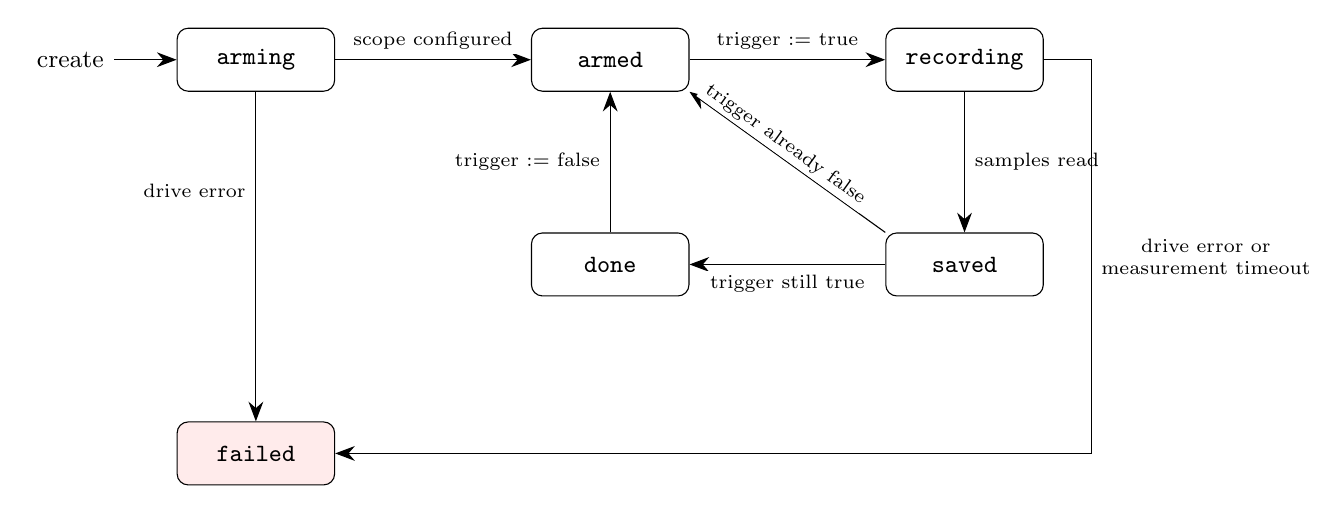
\begin{tikzpicture}[
    >={Stealth[length=2.5mm]},
    st/.style={rectangle, rounded corners, draw, minimum width=2.0cm, minimum height=0.8cm, font=\ttfamily\small},
    lbl/.style={font=\scriptsize, align=center, fill=white, inner sep=1.5pt},
  ]
  % Normal flow: top row left to right, then back along the bottom row.
  \node[st] (arming)    at (0, 0)    {arming};
  \node[st] (armed)     at (4.5, 0)  {armed};
  \node[st] (recording) at (9.0, 0)  {recording};
  \node[st] (saved)     at (9.0, -2.6) {saved};
  \node[st] (done)      at (4.5, -2.6) {done};
  \node[st, fill=red!8] (failed) at (0, -5.0) {failed};

  \draw[<-] (arming.west) -- ++(-0.8, 0) node[left, font=\small] {create};

  \draw[->] (arming) -- node[lbl, above=2pt] {scope configured} (armed);
  \draw[->] (armed) -- node[lbl, above=2pt] {trigger := true} (recording);
  \draw[->] (recording) -- node[lbl, right=2pt] {samples read} (saved);
  \draw[->] (saved) -- node[lbl, below=2pt] {trigger still true} (done);
  \draw[->] (done) -- node[lbl, left=2pt] {trigger := false} (armed);
  \draw[<-] (armed.south east) -- node[lbl, sloped, above, pos=0.45] {trigger already false} (saved.north west);

  % Failures run along the outside of the diagram.
  \draw[->] (arming) -- node[lbl, left=2pt, pos=0.3] {drive error} (failed);
  \draw[->] (recording.east) -- ++(0.6, 0) |- node[lbl, pos=0.25, right=2pt] {drive error or\\measurement timeout} (failed.east);
\end{tikzpicture}
\end{center}

A \dl{DELETE} (Data Layer \emph{remove}) is accepted in every state, including
\dl{failed}, and ends the capture.

\begin{center}
\small
\begin{tabularx}{\textwidth}{@{}>{\ttfamily}l X c c@{}}
\toprule
\normalfont State & What is happening & \dl{ready} & \dl{done} \\
\midrule
arming    & Connecting to the drive and writing the scope settings & false & false \\
armed     & Scope running, waiting for the trigger                 & true  & false \\
recording & Trigger fired; waiting for the scope memory to fill, then reading samples & false & false \\
saved     & Samples read; result being stored (short, transient)  & false & false \\
done      & Trace available on \dl{capture}                       & false & true  \\
failed    & Unrecoverable error or timeout; reason on \dl{error}   & false & false \\
\bottomrule
\end{tabularx}
\end{center}

Rules:
\begin{itemize}[nosep]
  \item \dl{measurement\_timeout\_ms} is measured from the trigger. If the trace
        is not complete by then, the capture moves to \dl{failed}.
  \item \dl{failed} is final. Nothing is cleaned up automatically; the capture
        (and its drive reservation) stays until the client deletes it.
  \item After writing \dl{trigger = false} in \dl{done}, the service re-arms the
        scope. \dl{ready} becomes \dl{true} once the drive confirms; until then
        the state is still \dl{done}.
\end{itemize}

%=====================================================================
\section{Data Formats}
%=====================================================================

\subsection{ScopeConfig (create request)}

\begin{center}
\small
\begin{tabularx}{\textwidth}{@{}>{\ttfamily}l l X@{}}
\toprule
\normalfont Field & Type & Meaning and validation \\
\midrule
drive\_ip\_address     & string    & Drive IPv4 address, four dotted octets. \\
signals                & [string]  & One SERCOS IDN per scope channel, form \dl{S-x-xxxx} or \dl{P-x-xxxx}. At least one. \\
time\_resolution\_us   & uint32    & Sample interval in \textmu s (drive P-0-0031). Must be $> 0$. \\
memory\_size           & uint32    & Number of samples per channel (drive P-0-0032). Must be $> 0$. \\
pre\_trigger\_percent  & ubyte     & Share of the memory recorded before the trigger, 0--100. \\
measurement\_timeout\_ms & uint32  & Time allowed from trigger to finished trace. Must be $> 0$. \\
\bottomrule
\end{tabularx}
\end{center}

Example, shown as JSON (the format used by \dl{DriveOscopeClient}; on the
Data Layer the body is the \dl{ScopeConfig} FlatBuffer):

\begin{lstlisting}[language=json]
{
  "drive_ip_address": "192.168.0.1",
  "signals": [ "S-0-0040", "S-0-0051" ],
  "time_resolution_us": 4000,
  "memory_size": 4096,
  "pre_trigger_percent": 20,
  "measurement_timeout_ms": 60000
}
\end{lstlisting}

\subsection{ScopeCapture (recorded trace)}

\begin{center}
\small
\begin{tabularx}{\textwidth}{@{}>{\ttfamily}l l X@{}}
\toprule
\normalfont Field & Type & Meaning \\
\midrule
captured\_at          & string   & Time of the trigger, ISO 8601 with UTC offset. \\
drive\_ip\_address    & string   & Drive the trace came from. \\
time\_resolution\_us  & uint32   & Sample interval used. \\
memory\_size          & uint32   & Memory size used. \\
pre\_trigger\_percent & ubyte    & Pre-trigger share used. \\
pre\_trigger\_samples & uint32   & Samples actually recorded before the trigger (see below). \\
drive\_p0032          & uint32   & P-0-0032 read back from the drive after configuration. \\
drive\_p0033          & uint32   & P-0-0033 read back from the drive after configuration: the number of samples recorded after the trigger. \\
time\_us              & [int32]  & Time of each sample relative to the trigger; negative values are before the trigger. \\
channels              & [Channel] & One entry per configured signal. \\
\midrule
Channel.index         & ubyte    & Channel number, starting at 1, in the order of \dl{signals}. \\
Channel.signal        & string   & SERCOS IDN recorded on this channel. \\
Channel.values        & [float]  & One value per entry in \dl{time\_us}. Up to \dl{memory\_size} values (see below). \\
\bottomrule
\end{tabularx}
\end{center}

\paragraph{Number of samples and the time axis.}
The drive returns only the samples it actually recorded. The part after the
trigger is always complete (\dl{drive\_p0033} samples). The part before the
trigger is only complete if the scope was armed long enough before the trigger,
that is at least
$(\text{memory\_size} - \text{drive\_p0033}) \cdot \text{time\_resolution\_us}$.
A trigger fired sooner gives a shorter trace with less pre-trigger history.
Therefore
\begin{gather*}
  \text{pre\_trigger\_samples} = N - \text{drive\_p0033}\\
  \text{time\_us}[i] = \bigl(i - \text{pre\_trigger\_samples}\bigr)\cdot \text{time\_resolution\_us},
  \qquad i = 0,\dots,N-1
\end{gather*}
where $N$ is the number of samples returned, so the sample at the trigger has
time 0. Example with \dl{memory\_size} 4096, 20\,\% pre-trigger and 4\,ms
resolution (\dl{drive\_p0033} = 3276): triggering right after arming returned
3311 samples (35 before the trigger); triggering 12\,s after arming returned
all 4096 (820 before the trigger).

To get the full pre-trigger history, wait at least that long after \dl{ready}
becomes \dl{true} before writing the trigger (UC3).

%=====================================================================
\section{Use Cases}
%=====================================================================

The code fragments use the .NET Data Layer client set up in the
Prerequisites section. \dl{captureAddress} is the value returned by the create
request, for example:

\begin{center}
\small\dl{ctrlx-drive-oscope/captures/7e85ebde-8b45-4f59-afce-acbfb33a446d}
\end{center}

%---------------------------------------------------------------------
\begin{usecase}{UC1: Create a capture}
\ucfield{Goal}{Configure the oscilloscope of one drive.}
\ucfield{Precondition}{No other capture exists for the same drive IP address.}
\ucfield{Postcondition}{A capture exists in state \dl{arming}; its address is known.}

\textbf{Steps}
\begin{enumerate}[nosep]
  \item Build a \dl{ScopeConfig} FlatBuffer.
  \item Send a Data Layer \emph{create} on \capsroot{} with the FlatBuffer as argument.
  \item On \res{DL\_OK}, the reply value is the new capture's address
        (\dl{ctrlx-drive-oscope/captures/\{id\}}). Keep it for all later requests.
\end{enumerate}

\begin{lstlisting}[language={[Sharp]C}]
var config = new ScopeConfigT {
    DriveIpAddress = "192.168.0.1",
    Signals = ["S-0-0040", "S-0-0051"],
    TimeResolutionUs = 4000, MemorySize = 4096,
    PreTriggerPercent = 20, MeasurementTimeoutMs = 60000,
};
var builder = new FlatBufferBuilder(Variant.DefaultFlatbuffersInitialSize);
builder.Finish(ScopeConfig.Pack(builder, config).Value);

var (result, location) = client.Create("ctrlx-drive-oscope/captures",
                                       new Variant(builder));
if (result.IsBad()) { /* DL_FAILED: invalid config or drive already in use */ }
string captureAddress = location.ToString();
\end{lstlisting}

\textbf{Failure:} \res{DL\_FAILED} when the config breaks a validation rule,
when the body is not a \dl{ScopeConfig} FlatBuffer, or when another capture
already uses the drive. The capture is not created. The service log states the
exact reason.

\textbf{Note:} the create returns before the drive is contacted. A wrong but
well-formed drive address is only detected afterwards; see UC2.
\end{usecase}

%---------------------------------------------------------------------
\begin{usecase}{UC2: Wait until the scope is armed}
\ucfield{Goal}{Know when the trigger can be fired.}
\ucfield{Precondition}{UC1 succeeded.}
\ucfield{Postcondition}{\dl{ready} is \dl{true}, state \dl{armed}.}

\textbf{Steps}
\begin{enumerate}[nosep]
  \item Poll \dl{\{id\}/ready} (for example every 200\,ms).
  \item On every poll where \dl{ready} is \dl{false}, also read \dl{\{id\}/state}.
        If it is \dl{failed}, read \dl{\{id\}/error}, report it and go to UC6.
  \item Use a client-side time limit (for example 30\,s) for drives that never
        answer.
\end{enumerate}

\begin{lstlisting}[language={[Sharp]C}]
while (true) {
    var (r, ready) = client.Read($"{captureAddress}/ready");
    if (r.IsGood() && ready.ToBool()) break;
    var (s, state) = client.Read($"{captureAddress}/state");
    if (s.IsGood() && state.ToString() == "failed") { /* read error, delete */ }
    await Task.Delay(200);
}
\end{lstlisting}
\end{usecase}

%---------------------------------------------------------------------
\begin{usecase}{UC3: Record and read one trace}
\ucfield{Goal}{Fire the trigger and get the recorded samples.}
\ucfield{Precondition}{State \dl{armed} (UC2).}
\ucfield{Postcondition}{State \dl{done}; the trace has been read.}

\textbf{Steps}
\begin{enumerate}[nosep]
  \item For a full pre-trigger history, wait at least
        $(\text{memory\_size} - \text{drive\_p0033}) \cdot \text{time\_resolution\_us}$
        after \dl{ready} became \dl{true} (Section~5.2).
  \item Write \dl{true} to \dl{\{id\}/trigger}. The service raises the scope's
        manual trigger; \dl{captured\_at} is set to this moment.
  \item Poll \dl{\{id\}/done} until it is \dl{true}, checking \dl{state} for
        \dl{failed} as in UC2. Allow at least \dl{measurement\_timeout\_ms}
        plus a margin for reading the samples.
  \item Read \dl{\{id\}/capture} and decode it as a \dl{ScopeCapture}.
        Reading is repeatable while the state is \dl{done}.
\end{enumerate}

\begin{lstlisting}[language={[Sharp]C}]
client.Write($"{captureAddress}/trigger", new Variant(true));
// ... poll {id}/done until true ...
var (r, value) = client.Read($"{captureAddress}/capture");
ScopeCaptureT trace = ScopeCapture.GetRootAsScopeCapture(value.ToFlatbuffers()).UnPack();
foreach (ChannelT channel in trace.Channels)
    Console.WriteLine($"{channel.Signal}: {channel.Values.Count} samples");
\end{lstlisting}

\textbf{Failures:}
\begin{itemize}[nosep]
  \item Writing the trigger returns \res{DL\_FAILED} while the state is
        \dl{arming} or \dl{failed}: the scope settings are not on the drive.
  \item The drive reports a scope error, or the trace is not complete within
        \dl{measurement\_timeout\_ms}: the state becomes \dl{failed}.
  \item Reading \dl{capture} before \dl{done} returns \res{DL\_FAILED}.
\end{itemize}
\end{usecase}

%---------------------------------------------------------------------
\begin{usecase}{UC4: Record another trace with the same settings}
\ucfield{Goal}{Re-arm without creating a new capture.}
\ucfield{Precondition}{State \dl{done} (UC3), trace read if needed.}
\ucfield{Postcondition}{State \dl{armed}; continue with UC3.}

\textbf{Steps}
\begin{enumerate}[nosep]
  \item Write \dl{false} to \dl{\{id\}/trigger}.
  \item Wait for \dl{ready} as in UC2. \dl{done} becomes \dl{false} when the
        scope is armed again.
  \item Continue with UC3.
\end{enumerate}

\textbf{Important:} re-arming discards the previous trace. Read
\dl{\{id\}/capture} before writing \dl{false}.

\textbf{Variant:} if \dl{false} is written while the trace is still recording,
the service skips \dl{done} and goes straight back to \dl{armed} after the
samples are read. The trace of that recording cannot be read.
\end{usecase}

%---------------------------------------------------------------------
\begin{usecase}{UC5: Monitor a capture}
\ucfield{Goal}{Show the progress of a capture, for example in an HMI.}

\textbf{Steps}
\begin{itemize}[nosep]
  \item Read \dl{\{id\}/state} for the current lifecycle state.
  \item Read \dl{\{id\}/trigger} for the last trigger value written.
  \item Browse \capsroot{} to list all existing captures.
\end{itemize}
\end{usecase}

%---------------------------------------------------------------------
\begin{usecase}{UC6: Delete a capture}
\ucfield{Goal}{Stop the capture and free the drive.}
\ucfield{Precondition}{The capture exists (any state).}
\ucfield{Postcondition}{The capture's nodes are gone; the drive is released shortly after.}

\textbf{Steps}
\begin{enumerate}[nosep]
  \item Send a Data Layer \emph{remove} on the capture address.
  \item \res{DL\_OK} confirms the request. The capture disappears from the
        Data Layer immediately; further requests on its address return
        \res{DL\_INVALID\_ADDRESS}.
\end{enumerate}

\begin{lstlisting}[language={[Sharp]C}]
DLR_RESULT removed = client.Remove(captureAddress);
\end{lstlisting}

\textbf{Behaviour:} the delete is fire and forget. The service answers at once
and the capture's worker stops and closes the drive connection in the
background. Until that has finished (normally well under a second, at most
about 8\,s if the drive does not respond) the drive stays reserved, and a
create for the same drive returns \res{DL\_FAILED}. Retry the create after a
short delay.

\textbf{Always delete} captures you no longer need, including failed ones.
Nothing is cleaned up automatically, and a capture blocks its drive for as long
as it exists.
\end{usecase}

%---------------------------------------------------------------------
\begin{usecase}{UC7: Recover from a failed capture}
\ucfield{Goal}{Find out why a capture failed and try again.}
\ucfield{Precondition}{\dl{\{id\}/state} reads \dl{failed}.}

\textbf{Steps}
\begin{enumerate}[nosep]
  \item Read \dl{\{id\}/error} for the reason (for example a drive connection
        error, a parameter that could not be written, or a measurement timeout).
  \item Delete the capture (UC6).
  \item Fix the cause (drive address, signal IDNs, timeout) and create a new
        capture (UC1).
\end{enumerate}
\end{usecase}

%=====================================================================
\section{Using the Command Line Client}
%=====================================================================

\dl{src/DriveOscopeClient} runs UC1 to UC4 and UC6 from a PC. It reads a
\dl{ScopeConfig} as JSON (snake\_case keys, as in the example above), creates
the capture, waits until it is armed, fires the trigger when Enter is pressed,
saves each trace as JSON, re-arms, and deletes the capture when it exits.

\begin{lstlisting}[language=bash]
dotnet run --project src/DriveOscopeClient -- scopeConfig.json \
    --core-ip 192.168.1.1 --ssl-port 443 \
    --user boschrexroth --password boschrexroth --output output
\end{lstlisting}

All options are optional; the values shown are the defaults. Without a config
path, \dl{scopeConfig.json} next to the executable is used. Each trace is
written to the output folder as \dl{scope\_yyyyMMdd\_HHmmss.json}.

%=====================================================================
\section{Result Code Reference}
%=====================================================================

\begin{center}
\small
\begin{tabularx}{\textwidth}{@{}l l X@{}}
\toprule
Request & Result & Cause \\
\midrule
Create \dl{captures}        & \res{DL\_OK}             & Capture created; value is its address \\
                            & \res{DL\_FAILED}         & Invalid config, not a \dl{ScopeConfig} FlatBuffer, or drive already in use \\
Create elsewhere            & \res{DL\_UNSUPPORTED}    & Only \dl{captures} accepts create \\
Read \dl{\{id\}/\dots}      & \res{DL\_INVALID\_ADDRESS} & Unknown or deleted \dl{capture\_id}, or unknown leaf \\
Read \dl{\{id\}/capture}    & \res{DL\_FAILED}         & State is not \dl{done} \\
Write \dl{\{id\}/trigger}   & \res{DL\_OK}             & Accepted; value echoed back \\
                            & \res{DL\_FAILED}         & State is \dl{arming} or \dl{failed} \\
                            & \res{DL\_INVALID\_VALUE} & Value is not a bool (or \dl{\{"trigger": true\}} JSON string) \\
Write elsewhere             & \res{DL\_UNSUPPORTED}    & Only \dl{trigger} is writable \\
Remove \dl{\{id\}}          & \res{DL\_OK}             & Delete accepted; cleanup runs in the background \\
                            & \res{DL\_INVALID\_ADDRESS} & Unknown or already deleted \dl{capture\_id} \\
\bottomrule
\end{tabularx}
\end{center}

\paragraph{Trigger value formats.}
The trigger accepts a Data Layer \dl{bool}. For clients that can only send
text, a string containing the JSON object \dl{\{ "trigger": true \}} (or
\dl{false}) is accepted as well.

\end{document}
